\section{Motivation}
\label{sec:motivation}
\subsection{Distributed Triangle Listing for Massive Graphs}
Graphs arise naturally in many real-world applications such as social networks, bio-medical networks, and communication networks.
In these applications, the graph can often be massive involving billions of vertices and edges.
For example,   Facebook's  social network involves more than 1.23 billion users (vertices), and more than 208 billion friendships (edges).
Such massive graphs can easily exceed the available memory of a single commodity computer.
That is why distributed analysis on massive graphs has become an important research area in recent years \cite{Pregel,PowerGraph}.

{\em Triangle listing}---which involves listing all triangles in a given graph---is well identified as a building-block operation
 in many graph analysis and mining techniques~\cite{Eckmann_Moses_2002, Khuller_Saha_2009}. 
First, several graph metrics can be directly obtained from triangle listing, e.g., {\em clustering coefficient} and {\em transitivity}. 
Such graph metrics have wide applications including quantifying graph density, detecting spam pages in web graphs, and measuring 
content quality in social networks~\cite{Becchetti_Boldi_Castillo_Gionis_2008}. 
Moreover, triangle listing has a broad range of applications including the discovery of dense sub-graphs~\cite{Khuller_Saha_2009}, 
study of motif occurrences~\cite{Milo_Shen-Orr_Itzkovitz_Kashtan_Chklovskii_2002}, 
and uncovering of hidden thematic relations in the web~\cite{Eckmann_Moses_2002}. 
%
There is another well-known and closely-related problem to triangle listing, which is the {\em triangle counting} problem. 
Clearly, solving the triangle listing problem would automatically solve triangle counting, but not vice versa.  
Compared to triangle counting, triangle listing serves a broader range of applications. 
For example, Motif identification~\cite{Milo_Shen-Orr_Itzkovitz_Kashtan_Chklovskii_2002},   
community detection~\cite{Berry_Hendrickson_LaViolette_Phillips_2011}, and dense subgraphs~\cite{Khuller_Saha_2009} 
are all dependent on the more complex {\em triangle listing} problem. 

Several techniques have been proposed for processing web-scale graphs including 
streaming algorithms~\cite{Becchetti_Boldi_Castillo_Gionis_2008,Buriol_Frahling_Leonardi_2006}, 
external-memory algorithms~\cite{H14,Kim_Han_Lee_Park_Yu_2014,GraphChi},
 and distributed parallel algorithms~\cite{Patric,Suri_Vassilvitskii_2011}. 
The streaming algorithms are limited to the {\em approximate triangle counting} problem. 
External-memory algorithms exploit asynchronous I/O and multi-core parallelism for efficient triangle listing~\cite{GraphChi,TurboGraph,H14}. 
In spite of achieving an impressive performance, external-memory approaches assume that the input graphs are in a centralized storage, 
which is not the case for many emerging applications that generate graphs distributed in nature. 
Even more seriously, external-memory approaches cannot easily scale up in terms of computing resources and parallelization degree.
Algorithm~\cite{Suri_Vassilvitskii_2011} presents a parallel algorithm for exact triangle counting using the MapReduce framework. 
The algorithm proposes a partitioning scheme that improves the memory requirements to some extent, yet it still suffers from a huge communication cost. 
Algorithm \cite{Patric} presents an efficient MPI-based distributed memory algorithm on the basis of~\cite{Suri_Vassilvitskii_2011} with load balancing techniques. 
However, as a memory-based algorithm, it suffers from memory limitations. 

In addition to these techniques, several distributed and specialized graph frameworks have been recently 
proposed as general-purpose graph processing engines~\cite{Pregel,PowerGraph,Gonzalez_Xin_Dave_Crankshaw_2014}.
However, most of these frameworks are  customized for iterative graph processing where distributed computations can be kept 
in-memory for faster subsequent iterations. However, the triangle listing algorithms are not iterative and would not make use of these optimizations. 

\subsection{Uncertain Graph Anonymization}
Network data has become increasingly important in recent years of the greater importance of various application domains such as Web, social network, biological networks, and communication networks. The semantics and the interpretation of the nodes and the links may vary with application domain, {\eg}, in a social network node can represent individuals and their connection captures friendship, while in a protein-to-protein network (PPI) nodes are proteins and connections refer to their interactions. These graph data carries valuable information and are analyzed in various ways to exact knowledge. For example, social networks provide significant insight into the psychological behavior of individuals or PPI networks are widely studied to elucidate the mechanism of diseases. 

In the same time, the existence of the relationship between two entities is uncertain due to noisy measurements and inference model. For instance, in PPI networks, since the interactions (edges) are derived through noisy and error-prone experiments, each edge is associated with an uncertainty value~\cite{Krogan_Global_2006}. In large social networks, uncertainty arises for various reasons~\cite{Adar_Managing_2007,Kempe_Maximizing_2003}. The edge probability may denote the \emph{influence} of one person on another~\cite{Kempe_Maximizing_2003}. Incorporating uncertainty to graphs lead to uncertain graphs (also called probabilistic graphs), whose edges are labeled with a probability of existence. This probability represents the confidence that the relation (the edge) holds in reality. The use of such information can enhance the effectiveness of graph mining algorithms because  the uncertainty provides a guidance in the use of different possible worlds during the mining process. Given the wide spectrum of application domains, querying and mining uncertain graphs has received considerable attention recently. 

Various agencies and data owners are increasingly sharing their uncertain graphs with third-party analysts, which immediately raises the big concern of data privacy.  An adversary may leverage any available auxiliary  information, e.g.,  node degrees, neighborhoods of breached nodes, to reveal the identities of the nodes in  the release graph \cite{Hay_Anonymizing_2007}. 
Such privacy vulnerability is a big barrier preventing the sharing, analytics, and the extraction of useful insights from these graphs. 

Before publishing, the graph needs to be anonymized to prevent potential re-identification attacks. Numerous graph anonymization techniques have been proposed in the literature to address this challenge~\cite{Liu_Towards_2008,Boldi_Injecting_2012, Mittal_Preserving_2013,Nguyen_Anonymizing_2015}. These anonymization techniques aim at minimizing the disclosure risk of private information by modifying graph at some level. However, these conventional methods have mainly focused on {\em deterministic graphs}, where the edges' presence is known with certainty.  In contrast, in uncertain graphs, the edges carry probabilities of their existence,  which makes the privacy-preservation problem far more different because of the incorporation of uncertainty in the de-anonymization process. 

% \begin{figure}[t!]
%     \centering 
%     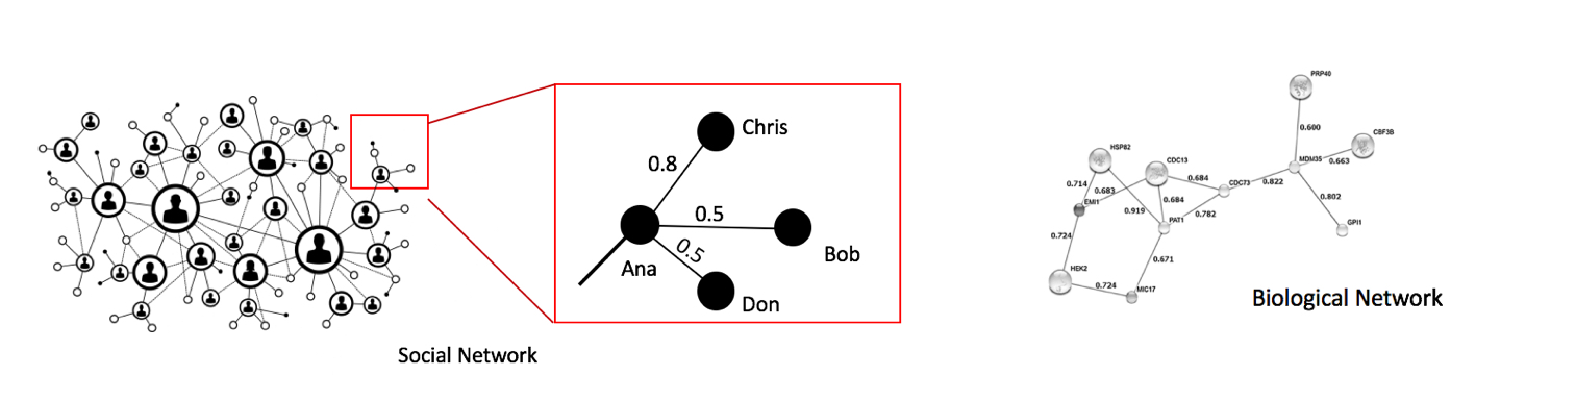
\includegraphics[scale=0.5]{figures/Intr/prevalenceUncertain.eps}
%     \caption{\small{The prevalence of uncertain graphs in real applications}}
% \end{figure}

\begin{figure}[t!]
    \centering 
    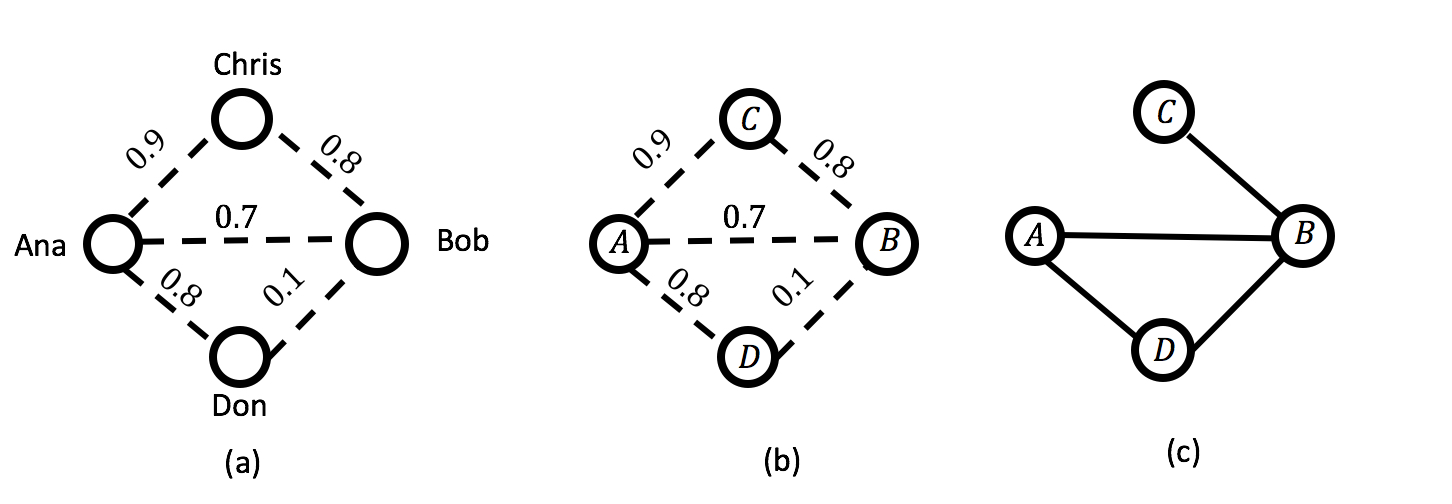
\includegraphics[scale=0.5]{figures/Intr/uncertainGraphExample.eps}
    \caption{\small{(a) The original uncertain graph (b) The naive anonymized version of uncertain graph with 5 edges and $2^{5}=32$ possible world} (c) One possible world: $G=\lbrace(AB),(AD),(BC),(BD) \rbrace$. The probability of $G$ is $Pr(G)=p(A,B) (1-p(A,c)) p(A,D) p(B,C) p(B,D)=0.00448$.}
    \label{fig:intr:uncertainGraph}
\end{figure}

Compared to deterministic graphs, the publishing of uncertain graphs reveals \textbf{additional} information--associated edge uncertainty which can be used by the adversary to re-identify some entities in the released uncertain graph. To gain more intuition on uncertain graph model and the difference in structural privacy attack, we present a simple example. Consider the release uncertain graph shown in Figure~\ref{fig:intr:uncertainGraph}. Each edge is associated with the probability of being present. Possible instantiations of this graph are commonly referred to as \emph{worlds}. In our example, there are $2^5=32$ possible worlds. The probability of a world can be calculated based on the probability of its edges as shown in the example in Figure~\ref{fig:intr:uncertainGraph}. Suppose the adversary has the external information, {\ie}, {\em Ana} has a degree of $3$ with high probability in the original graph. After the calculation of the probability that nodes has the degree of $3$ in the release uncertain graph as shown in the example in Figure~\ref{fig:intr:uncertainGraph}, the adversary could know that posterior probability that {\em Ana} is possible node $a$ is around 0.9 and is node $d$ is around 0.1. Clearly, it leads to the disclosure of node identity. To best of our knowledge, uncertain graph anonymization problem remains unexplored. 


